\chapter{\subspacesTitle}\label{subspacesspanning}

It is time to study vector spaces more carefully and return to  some fundamental questions:

\begin{enumerate}
\item \emph{Subspaces}: When is a subset of a vector space itself a vector space?  (This is the notion of a \emph{subspace}.)

\item \emph{Linear Independence}: Given a collection of vectors, is there a way to tell whether they are independent, or if one is a ``linear combination'' of the others? 

\item \emph{Dimension}: Is there a consistent definition of how ``big'' a vector space is?

\item \emph{Basis}:  How do we label vectors?  Can we write any vector as a sum of some basic set of vectors?  How do we change our point of view from vectors labeled one way to vectors labeled in another way?
\end{enumerate}
\index{Subspace!notion of}\index{Linear independence!concept of}\index{Dimension!notion of}\index{Basis!concept of}
Let's start at the top!

\section{Subspaces}

\begin{definition}
We say that a subset $U$ of a vector space $V$ is a {\bf subspace}\index{Subspace} of $V$ if $U$ is a vector space under the inherited addition and scalar multiplication operations of $V$. 
\end{definition}

\begin{example}
Consider a plane $P$ in $\Re^3$ through the origin:
\[
ax+by+cz=0.
\]

\begin{center}
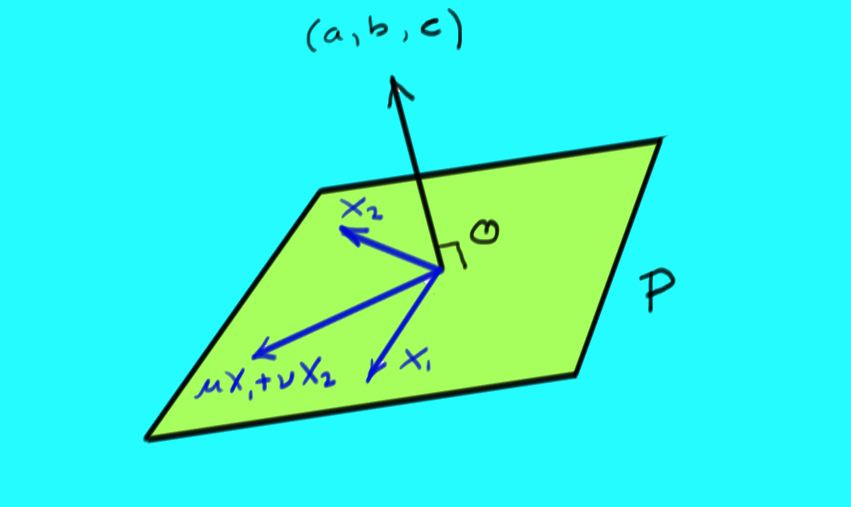
\includegraphics[scale=.3]{\subspacesPath/subspace_plane.jpg}
\end{center}
This equation can be expressed as the homogeneous system $\rowvec{a & b & c}\colvec{x\\y\\z}=0$, or $MX=0$ with $M$ the matrix $\rowvec{a & b & c}$.  If $X_1$ and $X_2$ are both solutions to $MX=0$, then, by linearity of matrix multiplication, so is $\mu X_1 + \nu X_2$:
\[
M(\mu X_1 + \nu X_2) = \mu MX_1 + \nu MX_2 = 0.
\]
So $P$ is closed under addition and scalar multiplication.  Additionally, $P$ contains the origin (which can be derived from the above by setting $\mu=\nu=0$).  All other vector space requirements hold for $P$ because they hold for all vectors in $\Re^3$.
\end{example}


%\begin{figure}
%\begin{center}
%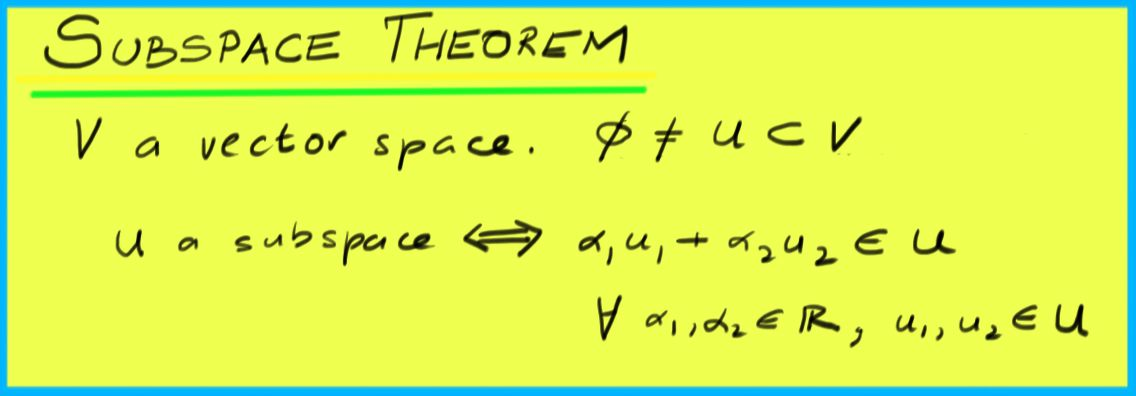
\includegraphics[scale=.33]{\subspacesPath/subspace_thm.jpg}
%\end{center}
%\end{figure}

\begin{theorem}[\hypertarget{sst}{Subspace Theorem}]\index{Subspace theorem}\label{subspacetheorem}
Let $U$ be a non-empty subset of a vector space $V$.  Then $U$ is a subspace if and only if $\mu u_1 + \nu u_2 \in U$ for arbitrary $u_1, u_2$ in $U$, and arbitrary constants $\mu, \nu$.  
\end{theorem}

\begin{proof}
One direction of this proof is easy: if \(U\) is a subspace, then it is a vector space, and so by the additive closure and multiplicative closure properties of vector spaces, it has to be true that \(\mu u_1 + \nu u_2 \in U\) for all \(u_1,u_2\) in \(U\) and all constants constants \(\mu, \nu\).

The other direction is almost as easy: we need to show that if \(\mu u_1 + \nu u_2 \in U\) for all \(u_1, u_2\) in \(U\) and all constants \(\mu, \nu\), then \(U\) is a vector space. That is, we need to show that the \hyperref[vectorspace]{ten properties of vector spaces} are satisfied. We already know that the additive closure and multiplicative closure properties are satisfied. Further, \(U\) has all of the other eight properties  because \(V\) has them. \end{proof}

\noindent
Note that the requirements of the subspace theorem are often referred to as ``closure''\index{Closure}.

%From now on, w
We can use this theorem to check if a set is a vector space. That is, if we have some set \(U\) of vectors that come from some bigger vector space \(V\), to check if \(U\) itself forms a smaller vector space we need check only two things: 
\begin{enumerate}
\item If we add any two vectors in \(U\), do we end up with a vector in \(U\)?
\item If we multiply any vector in \(U\) by any constant, do we end up with a vector in \(U\)? 
\end{enumerate}
If the answer to both of these questions is yes, then \(U\) is a vector space. If not, \(U\) is not a vector space.

%\begin{center}\href{\webworkurl ReadingHomework15/1/}{Reading homework: problem \ref{subspacesspanning}.1}\end{center}
\Reading{SubspacesAndSpans}{1}


\section{Building Subspaces}

Consider the set 
\[
U= \left\{ \colvec{1\\0\\0}, \colvec{0\\1\\0} \right\} \subset \Re^3.
\]
Because $U$ consists of only two vectors, it clear that $U$ is \emph{not} a vector space, since any constant multiple of these vectors should also be in $U$.  For example, the $0$-vector is not in $U$, nor is $U$ closed under vector addition.

But we know that any two vectors define a plane:
\begin{center}
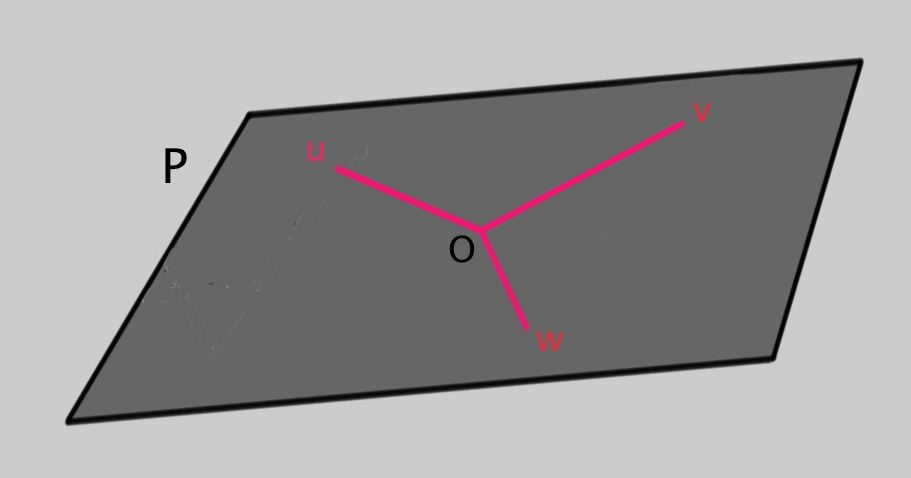
\includegraphics[scale=.3]{\subspacesPath/span_plane.jpg}
\end{center}
 In this case, the vectors in $U$ define the $xy$-plane in $\Re^3$.  We can view the $xy$-plane as the set of all vectors that arise as a linear combination of the two vectors in $U$.  We call this set of all linear combinations the \emph{span}\index{Span} of $U$:
\[
\spa(U)=\left\{ x \colvec{1\\0\\0}+y \colvec{0\\1\\0} \middle| x,y\in \Re \right\}.
\]
Notice that any vector in the $xy$-plane is of the form
\[
\colvec{x\\y\\0} = x \colvec{1\\0\\0}+y \colvec{0\\1\\0} \in \spa(U).
\]

\begin{definition}
Let $V$ be a vector space and $S=\{ s_1, s_2, \ldots \} \subset V$ a subset of~$V$.  Then the {\bf span of $S$}, denoted $\spa(S)$, is the set
\[
\spa(S):=\{ r^1s_1+r^2s_2+\cdots + r^Ns_N ~|~ r^i\in \Re, N\in \N \}.
\]
\end{definition}

That is, the span of \(S\) is the set of all finite linear combinations\footnote{Usually our vector spaces are defined over \(\mathbb{R}\), but in general we can have vector spaces defined over different base fields such as \(\mathbb{C}\) or \(\mathbb{Z}_2\). The coefficients \(r^i\) should come from whatever our base field is (usually \(\mathbb{R}\)).} of elements of \(S\). Any {\it finite} sum of the form ``a constant times \(s_1\) plus a constant times \(s_2\) plus a constant times \(s_3\) and so on'' is in the span of \(S\).\footnote{It is important that we only allow finitely many terms in our linear combinations; in the definition above, \(N\) must be a finite number. It can be any finite number, but it must be finite. We can relax the requirement that $S=\{s_1,s_2,\ldots\}$ and just let $S$ be any set of vectors. Then we shall write $\spa(S):=\{ r^1s_1+r^2s_2+\cdots + r^Ns_N ~|~ r^i\in \Re, s_i\in S, N\in \N, \}$
 }.

\begin{example}
Let $V=\Re^3$ and $X\subset V$ be the $x$-axis.  Let $P=\colvec{0\\1\\0}$, and set $$S=X \cup \{P\}\, .$$
The vector \(\colvec{2 \\ 3 \\ 0}\) is in \(\spa(S),\) because \(\colvec{2\\3\\0}=\colvec{2\\0\\0}+3\colvec{0\\1\\0}.\) Similarly, the vector \(\colvec{-12 \\ 17.5 \\ 0}\) is in \(\spa(S),\) because \(\colvec{-12\\17.5\\0}=\colvec{-12\\0\\0}+17.5\colvec{0\\1\\0}.\)
Similarly, any vector of the form
\[
\colvec{x\\0\\0}+y \colvec{0\\1\\0} = \colvec{x\\y\\0}
\]
is in \(\spa(S)\). On the other hand, any vector in \(\spa(S)\) must have a zero in the \(z\)-coordinate. (Why?) 
So $\spa(S)$ is the $xy$-plane, which is a vector space.  (Try drawing a picture to verify this!)
\end{example}

%\begin{center}\href{\webworkurl ReadingHomework15/2/}{Reading homework: problem \ref{subspacesspanning}.2}\end{center}
\Reading{SubspacesAndSpans}{2}

\begin{lemma}
For any subset $S\subset V$, $\spa(S)$ is a subspace of $V$.
\end{lemma}

\begin{proof}
We need to show that $\spa(S)$ is a vector space.

It suffices to show that $\spa(S)$ is closed under linear combinations.  Let $u,v\in \spa(S)$ and $\lambda, \mu$ be constants.  By the definition of $\spa(S)$, there are constants $c^i$ and $d^i$ (some of which could be zero) such that:
\begin{eqnarray*}
u & = & c^1s_1+c^2s_2+\cdots \\
v & = & d^1s_1+d^2s_2+\cdots \\
\Rightarrow \lambda u + \mu v & = & \lambda (c^1s_1+c^2s_2+\cdots ) + \mu (d^1s_1+d^2s_2+\cdots ) \\
& = & (\lambda c^1+\mu d^1)s_1 + (\lambda c^2+\mu d^2)s_2 + \cdots
\end{eqnarray*}
This last sum is a linear combination of elements of $S$, and is thus in $\spa(S)$.  Then $\spa(S)$ is closed under linear combinations, and is thus a subspace of~$V$.
\end{proof}

Note that this proof, like many proofs, consisted of little more than just writing out the definitions.



\begin{example}
For which values of $a$ does

\[
\spa \left\{ \colvec{1\\0\\a} , \colvec{1\\2\\-3} , \colvec{a\\1\\0}   \right\} = \Re^3?
\]
Given an arbitrary vector $\colvec{x\\y\\z}$ in $\Re^3$, we need to find constants $r^1, r^2, r^3$ such that 

\[
r^1 \colvec{1\\0\\a} + r^2\colvec{1\\2\\-3} +r^3 \colvec{a\\1\\0} = \colvec{x\\y\\z}.
\]
We can write this as a linear system in the unknowns $r^1, r^2, r^3$ as follows:

\[
\begin{pmatrix}
1 & 1 & a \\ 
0 & 2 & 1 \\
a & -3 & 0
\end{pmatrix}
\colvec{r^1\\r^2\\r^3}
= \colvec{x\\y\\z}.
\]
If the matrix $M=\begin{pmatrix}
1 & 1 & a \\ 
0 & 2 & 1 \\
a & -3 & 0
\end{pmatrix}$ is invertible, then we can find a solution 
\[
M^{-1}\colvec{x\\y\\z}=\colvec{r^1\\r^2\\r^3}
\]
for \emph{any} vector $\colvec{x\\y\\z} \in \Re^3$.

Therefore we should choose $a$ so that $M$ is invertible:  

\[
i.e.,\;  0 \neq \det M = -2a^2 + 3 + a = -(2a-3)(a+1). 
\]
Then the span is $\Re^3$ if and only if $a \neq -1, \frac{3}{2}$.
\end{example}

\Videoscriptlink{subspaces_and_spanning_sets_example.mp4}{Linear systems as spanning sets}{scripts_subspaces_and_spanning_sets_example}

Some other very important ways of building subspaces are given in the following examples.

\begin{example}
(The kernel of a linear map).\\[-2mm]

\noindent
Suppose $L:U\to V$ is a linear map between vector spaces. Then if
$$
L(u)=0=L(u')\, ,
$$
linearity tells us that
$$
L(\alpha u + \beta u') = \alpha L(u) + \beta L(u') =\alpha 0 + \beta 0 = 0\, .
$$
Hence, thanks to the subspace theorem,  the set of all vectors in $U$ that are mapped to the zero vector is a subspace of $V$.
It is called the kernel of $L$:
$$
{\rm ker} L:=\{u\in U| L(u) = 0\}\subset U.
$$
Note that finding a kernel means finding a solution to a homogeneous linear equation. 
\end{example}

\begin{example}
(The image of a linear map).\\[-2mm]

\noindent
Suppose $L:U\to V$ is a linear map between vector spaces. Then if
$$
v=L(u) \mbox{ and } v'=L(u')\, ,
$$
linearity tells us that
$$
\alpha v + \beta v' = \alpha L(u) + \beta L(u') =L(\alpha u +\beta u')\, .
$$
Hence, calling once again on the subspace theorem,  the set of all vectors in $V$ that are obtained as outputs of the
map $L$ is a subspace.
It is called the image of $L$:
$$
{\rm im} L:=\{L(u) \ |\  u\in U \}\subset V.
$$
\end{example}

\begin{example}
(An eigenspace of a linear map).\\[-2mm]

\noindent
Suppose $L:V\to V$ is a linear map and $V$ is a vector space. Then if
$$
L(u)=\lambda u \mbox{ and } L(v)=\lambda v\, ,
$$
linearity tells us that
$$
L(\alpha u + \beta v) = \alpha L(u) + \beta L(v) =\alpha L(u) + \beta L(v) =\alpha \lambda u  + \beta \lambda v = \lambda (\alpha u + \beta v)\, .
$$
Hence, again by subspace theorem, the set of all vectors in $V$ that
obey the {\it eigenvector equation} $L(v)=\lambda v$ is a subspace of $V$. 
It is called an eigenspace
$$
V_\lambda:=\{v\in V| L(v) = \lambda v\}.
$$
For most scalars $\lambda$, the only solution to $L(v) = \lambda v$ will be $v=0$, which yields the trivial subspace $\{0\}$.
When there are nontrivial solutions to $L(v)=\lambda v$, the number~$\lambda$ is called an eigenvalue, and carries
essential information about the map~$L$. 
\end{example}

Kernels, images and eigenspaces are discussed in great depth in chapters~\ref{kernelrank} and~\ref{eigenvalseigenvects}.


%\section*{References}
%Hefferon, Chapter Two, Section I.2: Subspaces and Spanning Sets
%\\
%Beezer, Chapter VS, Section S
%\\
%Beezer, Chapter V, Section LC
%\\
%Beezer, Chapter V, Section SS
%\\
%Wikipedia:
%\begin{itemize}
%\item \href{http://en.wikipedia.org/wiki/Linear_subspace}{Linear Subspace}
%\item \href{http://en.wikipedia.org/wiki/Linear_span}{Linear Span}
%\end{itemize}
%

\section{Review Problems}
{\bf Webwork:} 
\begin{tabular}{|c|c|}
\hline
Reading Problems & 
 \hwrref{SubspacesAndSpans}{1}, \hwrref{SubspacesAndSpans}{2}\\
 Subspaces &\hwref{SubspacesAndSpans}{3},
 \hwref{SubspacesAndSpans}{4},
 \hwref{SubspacesAndSpans}{5},
 \hwref{SubspacesAndSpans}{6}\\
 Spans &\hwref{SubspacesAndSpans}{7},
 \hwref{SubspacesAndSpans}{8}\\
  \hline
\end{tabular}






\begin{enumerate}

\item Let $D=\begin{pmatrix}
\lambda_1 & \mc0 \\
\mc0 & \lambda_2 \\
\end{pmatrix}$.
\begin{enumerate}
\item Write $D$ in terms of the vectors $e_1$ and $e_2$, and their transposes.
\item Suppose $P=\begin{pmatrix}
a & b \\
c & d \\
\end{pmatrix}$ is invertible.  Show that $D$ is similar to
\[
M=\frac{1}{ad-bc}\begin{pmatrix}
\lambda_1ad-\lambda_2bc & -(\lambda_1-\lambda_2)ab \\[1mm]
(\lambda_1-\lambda_2)cd & -\lambda_1bc + \lambda_2ad
\end{pmatrix}.
\]
\item Suppose the vectors $\rowvec{a,b}$ and $\rowvec{c,d}$ are orthogonal.  What can you say about $M$ in this case? (Hint: think about what \(M^T\) is equal to.)
\end{enumerate}

\phantomnewpage

\item \label{orthogprob} Suppose $S=\{v_1, \ldots, v_n \}$ is an \emph{orthogonal} (not orthonormal) basis for~$\Re^n$.  Then we can write any vector $v$ as $v=\sum_ic^iv_i$ for some constants $c^i$.  Find a formula for the constants $c^i$ in terms of $v$ and the vectors in~$S$.

\Videoscriptlink{orthonormal_bases_hint.mp4}{Hint}{scripts_orthonormal_bases_hint}
\phantomnewpage

\item \label{orthogprojprob} Let $u,v$ be linearly independent vectors in $\Re^3$, and $P=\spa \{ u,v\}$ be the plane spanned by $u$ and $v$.  
\begin{enumerate}
\item Is the vector $v^\bot := v-\frac{u\cdot v}{u\cdot u}u$ in the plane $P$?
\item  What is the (cosine of the) angle between $v^\bot$ and $u$?
\item %Given your solution to the above, 
How can you find a third vector perpendicular to both $u$ and $v^\bot$?
\item  Construct an orthonormal basis for $\Re^3$ from $u$ and $v$.
\item  Test your abstract formul\ae\ starting with 
\[
u=\rowvec{1 , 2 , 0} \text{ and } v=\rowvec{0 , 1 , 1}.
\]
\end{enumerate}

\Videoscriptlink{orthonormal_bases_hint3.mp4}{Hint}{scripts_orthonormal_bases_hint3}

\phantomnewpage



\item Find an orthonormal  basis for $\Re^4$ which includes $(1,1,1,1)$ using the following procedure:\\
\begin{enumerate} 
\item Pick a vector perpendicular to the vector 
$$v_1 =\colvec{1\\1\\1\\1}$$ from the solution set of the matrix equation $$v_1^Tx=0\, .$$ Pick the vector $v_2$ obtained from the standard Gaussian elimination procedure which is the coefficient of $x_2$.
\item Pick a vector perpendicular to both $v_1$ and $v_2$ from the solutions set of the matrix equation $$\colvec{v_1^T\\[1mm]v_2^T}x=0\, .$$ Pick the vector $v_3$ obtained from the standard Gaussian elimination procedure with $x_3$ as the coefficient. 
\item Pick a vector perpendicular to $v_1,v_2,$ and $v_3$ from the solution set of the matrix equation $$\colvec{v_1^T\\[1mm]v_2^T\\[1mm]v_3^T}x=0\, .$$  Pick the vector $v_4$ obtained from the standard Gaussian elimination procedure with $x_3$ as the coefficient. 
\item Normalize the four vectors obtained   above.
\end{enumerate}


\item Use the inner product $$f\cdot g := \int_0^1 f(x)g(x)dx$$  on the vector space $V={\rm span} \{1,x,x^2,x^3\}$ to perform the Gram-Schmidt procedure on the set of vectors $\{1,x,x^2,x^3\}$. 

\item Use the inner product $$f\cdot g := \int_0^{2\pi} f(x)g(x)dx$$  on the vector space $V={\rm span} \{\sin(x),\sin(2x),\sin(3x) \}$ to perform the Gram-Schmidt procedure on the set of vectors $\{\sin(x),\sin(2x),\sin(3x) \}$. \\
Try to build an orthonormal basis for the vector space $$\spa \{ \sin(nx)~| ~n\in \N \}\, .$$
%What do you suspect about the vector space $\spa \{ \sin(nx)~| ~n\in \N \}$?\\
%What do you suspect about the vector space $\spa \{ \sin(ax)~|~ a \in \Re \}$?
\item 
\begin{enumerate}
\item
Show that if $Q$ is an orthogonal $n\times n$ matrix, then $$u\dotprod v = (Qu)\dotprod (Qv)\, ,$$ for any $u,v\in \Re^n$. That is, $Q$ preserves the inner product. 
\item Does $Q$ preserve the outer product? 
\item  If the set of vectors $\{ u_1,\dots,u_n\}$ is orthonormal and $\{ \lambda_1,\cdots,\lambda_n\}$ is a set of numbers, 
then what are the eigenvalues and eigenvectors of the matrix
$M=\sum_{i=1}^n \lambda_i u_i u_i^T$? 
\item How would the eigenvectors and eigenvalues of this matrix change if we replaced  $\{ u_1,\dots,u_n\}$ by $\{ Qu_1,\dots,Q u_n\}$?
\end{enumerate}


\item Carefully write out the Gram-Schmidt procedure for the set of vectors 
$$\left\{ \colvec{1\\1\\1}, \colvec{1\\-1\\1}, \colvec{1\\1\\-1} \right\} \, .$$ Is it possible to rescale the second vector obtained in the procedure to a vector with integer components? 


\item 
\label{basisortho}
\begin{enumerate}
\item Suppose $u$ and $v$ are linearly independent.  Show that $u$ and $v^\perp$ are also linearly independent.  Explain why $\{u, v^\perp\}$ is a basis for $\spa \{u,v\}$.



\Videoscriptlink{gram_schmidt_and_orthogonal_complements_hint.mp4}{Hint}{gram_schmidt_and_orthogonal_complements_hint}

\item Repeat the previous problem, but with three independent vectors $u,v,w$
 where $v^\perp$ and $w^\perp$ are as defined by the Gram-Schmidt procedure. 
\end{enumerate}

\phantomnewpage


\item \label{QRprob} Find the $QR$ factorization of
$$
M=\begin{pmatrix}1&0&\phantom{\!-}2\\-1&2&0\\-1&-2&2
\end{pmatrix}\, .
$$

\phantomnewpage

\item Given any three vectors $u,v,w$, when do $v^\perp$ or $w^\perp$ of the Gram--Schmidt procedure vanish?

\phantomnewpage

\item For $U$ a subspace of $W$, use the subspace theorem to check that $U^\perp$ is a subspace of $W$.

\phantomnewpage


\phantomnewpage

\item %(Extra Credit) 
Let $S_n$ and $A_n$ define the space of $n \times n$ symmetric and anti-symmetric matrices, respectively. These are subspaces of the vector space $M^n_n$ of all $n\times n$ matrices. What is $\dim M^n_n$, $\dim S_n$, and $\dim A_n$? Show that $M^n_n = S_n + A_n$. Define an inner product on square matrices
$$
M\cdot N ={\rm tr} MN\, .
$$
Is $A_n^{\perp}=S_n$? Is $M^n_n = S_n \oplus A_n$?

%\emph{Hint: Note that $\dim S_n = \dim U_n$ where $U_n$ is the vector space of all $n \times n$ upper triangular matrices, and also note that $\dim A_n = \dim \widetilde{U}_n$ where $\widetilde{U}_n$ is the vector space of all strictly $n \times n$ upper triangular matrices (\emph{i.e.} the diagonal entries are all 0).}

\item The vector space $V={\rm span} \{ \sin(t),\sin(2t), \sin(3t) , \sin(3t)\}$ has an inner product: 
$$f\cdot g:=\int _0^{2\pi}f(t)g(t) dt\, .$$ Find the orthogonal compliment to $U={\rm span} \{ \sin(t)+\sin(2t) \}$ in $V$. Express $\sin(t)-\sin(2t)$ as  the sum of vectors from $U$ and $U^\perp$.

\end{enumerate}

\phantomnewpage



\newpage
